\documentclass[a4paper, 12pt]{article}

\usepackage[T1]{fontenc}
\usepackage[dvips]{epsfig}

\usepackage[latin1]{inputenc}

\usepackage[english]{babel}
%\usepackage{times}
\usepackage[dvips]{graphics}

\usepackage[]{vmargin}
\usepackage{url}
\usepackage[]{longtable}

\usepackage{natbib}
\bibpunct{(}{)}{;}{a}{,}{,}

%\usepackage{color}

\newcommand{\jel}{Jeliot}
\newcommand{\jelIII}{Jeliot~3}
\newcommand{\djava}{DynamicJava}
\newcommand{\p}[1]{\texttt{#1}}
\newcommand{\bu}[1]{\textsf{#1}}
\newcommand{\f}[1]{\textsf{#1}}


\setlength{\parindent}{0pt} \setlength{\parskip}{2ex}
\linespread{1.3}
%\sloppy
%\fussy

\setpapersize{A4}
\setmarginsrb{35mm}{30mm}{30mm}{20mm}{0pt}{0mm}{12pt}{13mm}


\title{\jel{} Program Animation System\\Internal Documentation\\\mbox{}\\\large{Version 3.2}}
\author{Niko Myller and Andr\'{e}s Moreno Garc\'{\i}a}
%\date{}

\begin{document}
% ----------------- Coverpage -------------------------------

\maketitle
\thispagestyle{empty}

% --- Alternative coverpage ---
%
%\vspace*{4cm}
%
%\vspace{2cm}
%
%{\LARGE \jel{} Program Animation System\\Internal Documentation}
%
%{\Large Version 3.2}
%
%\vspace{2cm}
%
%{\large Andr\'{e} Moreno-Garc\'{\i}a and Niko Myller}
%
%\vspace{\stretch{1}}
%
%{\large
%X.X.2003 \\ \\
%University of Joensuu \\
%Department of Computer Science\\
%Special Project in Computer Science\\
%Software Documentation
%}
%
%\vspace{1cm}
%
%\thispagestyle{empty} % no page numbering

\newpage

\thispagestyle{empty} % no page numbering
\vfil
Copyright \copyright{} 2003-2004  Niko Myller and Andr\'{e}s Moreno Garc\'{\i}a.
\bigskip

{\small Permission is granted to copy, distribute and/or modify this document
under the terms of the GNU Free Documentation License, Version 1.2
or any later version published by the Free Software Foundation;
with Invariant Section Appendix A GNU Free Documentation License,
no Front-Cover Texts, and no Back-Cover Texts.
A copy of the license is included in the section entitled ``GNU Free Documentation License''. }

{\emph \djava{}} is distributed under the terms of a BSD-like license:

\djava{} - Copyright \copyright 1999 Dyade

{\small Permission is hereby granted, free of charge, to any person
obtaining a copy of this software and associated documentation
files (the "Software"), to deal in the Software without restriction,
including without limitation the rights to use, copy, modify, merge,
publish, distribute, sublicense, and/or sell copies of the Software,
and to permit persons to whom the Software is furnished to do so,
subject to the following conditions: The above copyright notice and
this permission notice shall be included in all copies or substantial
portions of the Software. }

{\small THE SOFTWARE IS PROVIDED "AS IS", WITHOUT WARRANTY OF ANY KIND,
EXPRESS OR IMPLIED, INCLUDING BUT NOT LIMITED TO THE WARRANTIES OF
MERCHANTABILITY, FITNESS FOR A PARTICULAR PURPOSE AND NONINFRINGEMENT.
IN NO EVENT SHALL DYADE BE LIABLE FOR ANY CLAIM, DAMAGES OR OTHER
LIABILITY, WHETHER IN AN ACTION OF CONTRACT, TORT OR OTHERWISE, ARISING
FROM, OUT OF OR IN CONNECTION WITH THE SOFTWARE OR THE USE OR OTHER
DEALINGS IN THE SOFTWARE. }

{\small Except as contained in this notice, the name of Dyade shall not be used
in advertising or otherwise to promote the sale, use or other dealings
in this Software without prior written authorization from Dyade. }

\vfil
\newpage

% ----------------- Generation of Table of Contents -------------

\thispagestyle{empty} % no page numbering

\setlength{\parskip}{0ex}

\tableofcontents
\newpage

\setlength{\parskip}{2ex}

% ----------------- Document begins ------------------------

\setcounter{page}{1}
\pagenumbering{arabic} % page numbering with arabic numbers

%Introduction
\section{Introduction}
\label{sec:Introduction}

\jel{} is a program animation system intended for teaching introductory
programming. Programs are animated fully or semi-automatically, requiring
no modifications or annotations on the part of the instructor or student.
While this limits the flexibility of the animation, \jel{} is extremely
simple to use so that it is easily accepted by true novices, as well as
by their teachers who do not have to invest in learning how to prepare
animations.

\jel{} is written in Java for portability and animates program that are
written in Java. \jel{} uses a modified version of \djava{} \citep{DJava}
(section~\ref{sec:DynamicJava}) as a front-end and
modified version of \jel{}~2000's animation engine
(section~\ref{sec:Visualization_Engine}) as its back-end. The user interface
was also adopted from \jel{}~2000 (sections~\ref{sec:Jeliot_Class} and
\ref{sec:User_Interface}).

\djava{} is a Java source code interpreter written in Java. This
application is open source and can be freely obtained from
\url{http://www.koala.ilog.fr/djava/}. At the moment, DynamicJava is
almost fully compliant with Java language specifications and supports
multi-threading.

To make these two separate systems communicate
(section~\ref{sec:Communications_Model}) with each other a new
intermediate code (section~\ref{sec:Intermediate_Code} and
Intermediate Language Specification) and intermediate code
interpreter (section~\ref{sec:Intermediate_Code_Interpreter}) were
designed. In this way the system should be more flexible for
modifications and new extensions
(sections~\ref{sec:Managing_Jeliot_3_System} and
\ref{sec:Extending_Jeliot_System}).

\subsection{History}

The first member of the \jel{} family of program animation systems was
called Eliot; it was developed by Erkki Sutinen and Jorma Tarhio and
their students at the University of Helsinki. Eliot was written in C
and used the Polka animation library. Later a version was written in
Java and the name was changed to \jel{}. (This version is now called
\jel{}~I to distinguish it from later versions.)

\jel{}~I was a flexible system: the user could choose the variables to
be animated, the graphical form of the animated elements and multiple
views of the same program. It proved too difficult for teaching novices,
so a new version called \jel{}~2000 was developed at the Weizmann Institute
of Science by Pekka Uronen under the supervision of Moti Ben-Ari.
A pedagogical experiment carried out by Ronit Ben-Bassat Levy proved
the effectiveness of \jel{} in teaching introductory programming.

\jel{}~2000 only implemented a very small subset of the Java language.
The current version \jel{}~3 is a re-implementation designed to
significantly extend the range of Java features that are animated,
in particular, to cover object-oriented programming. The design and
implementation was carried out at the University of Joensuu by
Niko Myller and Andr{\'{e}} Moreno-Garc{\'{\i}}a, under the supervision
of Moti Ben-Ari and Erkki Sutinen. For an extensive discussion of the
history of \jel{}, see \citep{Benari2002a}.

\subsection{Release Notes}
\label{sec:Release_Notes}

\paragraph{version 3.2} contains documentation and supports
inheritance, supports: inheritance of classes and \p{super()}
method calls at the beginning of a constructor.

\paragraph{version 3.1} supports objects creation and object method
calls. Line numbering was added for source code editor and viewer.
Supports:
\begin{itemize} \item User made classes, however,
inheritance is not yet supported. \item Constructor calls. \item
Object method calls. \item Object field access.
\end{itemize}


\paragraph{Version 3.01} is a maintenance release. Bugs of the initial
release were fixed. Support for \p{switch} statement was added.

\paragraph{Version 3.0} is the initial public release. Supports:
\begin{itemize}
\item Values of type \p{String}, all primitive types. \item
One-dimensional arrays with primitive types or strings as its
component type. \item Expressions including all unary and binary
operations except \p{instanceof}. \item All the control statements
(\p{if}, \p{while}, etc.) except \p{switch} statement and
conditional expression (\p{exp?exp1:exp2}). \item Method
invocation, including recursive invocation.
\end{itemize}

\paragraph{Not implemented:}
\begin{itemize}
\item Static variables. \item Calls to \p{super()} with
parameters. \item Super field accesses. \item Arrays with
components of reference type (except \p{String}). \item
Conditional expressions (\p{exp?exp1:exp2}). \item Array
initializers. \item Java 2 SDK API classes' methods cannot return
object or array types.
\end{itemize}

\newpage


\section{Managing \jel{} System}
\label{sec:Managing_Jeliot_3_System}

In this chapter we explain what are the system requirements of \jel{},
what files and directories different distributions contain and
how the source code distribution can be build. This will lead us to
the next chapter containing information about how to extend \jel{} system.

\subsection{System Requirements}
\label{sec:System_Requirements}

\subsection{End User Distribution}
\label{sec:End_User_Distribution}

\subsection{Source Code Distribution}
\label{sec:Source_Code_Distribution}

\subsubsection{Directory Hierarchy}

\jel{} is available as zip file containing all the sources
and files needed to build it. After unzipping the file we will
find the following directories:
\begin{description}
\item[\p{lib}] Contains the tools needed for the automated build process.
\item[\p{resources}] Contains information messages used by DynamicJava
to alert from errors.
\item[\p{src}] Contains the source code for \jel{}. It is divided into
the following subfolders.
\begin{description}
\item[\p{docs}] Contains the web pages that are used for the help page
and the about page. It also contains the licenses under which
\jel{} is distributed.
\item[\p{examples}] Contains the examples that will be available for users
of \jel{}, new examples can be added here.
\item[\p{images}] Those images used in the user interface of \jel{}.
\item[\p{jeliot}] All source files related to \jel{} visualization engine (\p{theatre}),
m-code interpretation (\p{ecode}) and the graphical user interface (\p{gui}).
\item[\p{koala}] The modified source code of \djava{}.
\end{description}
\end{description}

\subsubsection{How to Build Jeliot 3 From the Sources}

Being used to the build tool used by DynamicJava (Ant), it was
modified to build also \jel{}. Ant is a UNIX make-clone oriented
to build Java programs based on an XML configuration file \url{http://ant.apache.org}.
When unzipping the source code, three files will appear on the
destination directory:
\begin{description}
\item[build.xml] This file defines the possible targets and its tasks
that we want to perform with Ant. It includes some properties
to customize the output. For example, you can rename the minor
version of \jel{} by modyfing the property named minor. For adding
more targets you should refer to Ant manual page
(\url{http://ant.apache.com/manual/index.html}).
\item[build.bat and build.sh] These are the batch files that
will invoke Ant with one of the arguments (targets) that you
can provide to it:
\begin{description}
\item[compile] \jel{} source code will be compiled and classes obtained
will be located at classes subfolder. To run \jel{} from this
point you should enter the command java jeliot.Jeliot inside
the classes subfolder.
\item[dist] This argument will compile (if necessary), create the
jar files and zip them. This way we will obtain a binary zip
file of \jel{} Jeliot3\$\{minor\}.zip and another
zip file of \jel{} source code Jeliot3\$\{minor\}-src.zip.
These files are ready to be distributed without any modifications.
\item[clean] deletes every file created by the build tool.
\end{description}
\end{description}
Notice that you must set JAVA\_HOME to point at your Java Development
Kit installation.

A normal session could consist of the following commands:
\begin{verbatim}
c:\jeliot3> build compile
\end{verbatim}
The compiled class files are now in the folder classes.
\begin{verbatim}
c:\jeliot3> cd classes
c:\jeliot3\classes> java jeliot.Jeliot
\end{verbatim}
We can run Jeliot with the command above. But if we want to make a
distribution we need to do as follows and we will get two separate
distributions one with the compiled files and one with the source codes.
\begin{verbatim}
c:\jeliot3\classes> cd ..
c:\jeliot3> build dist
c:\jeliot3> cd Jeliot3
c:\jeliot3\Jeliot3> jeliot
\end{verbatim}


\newpage


%\section{Concept Design}
\label{sec:Concept_Design}

\begin{figure}[!htb]
\begin{center}
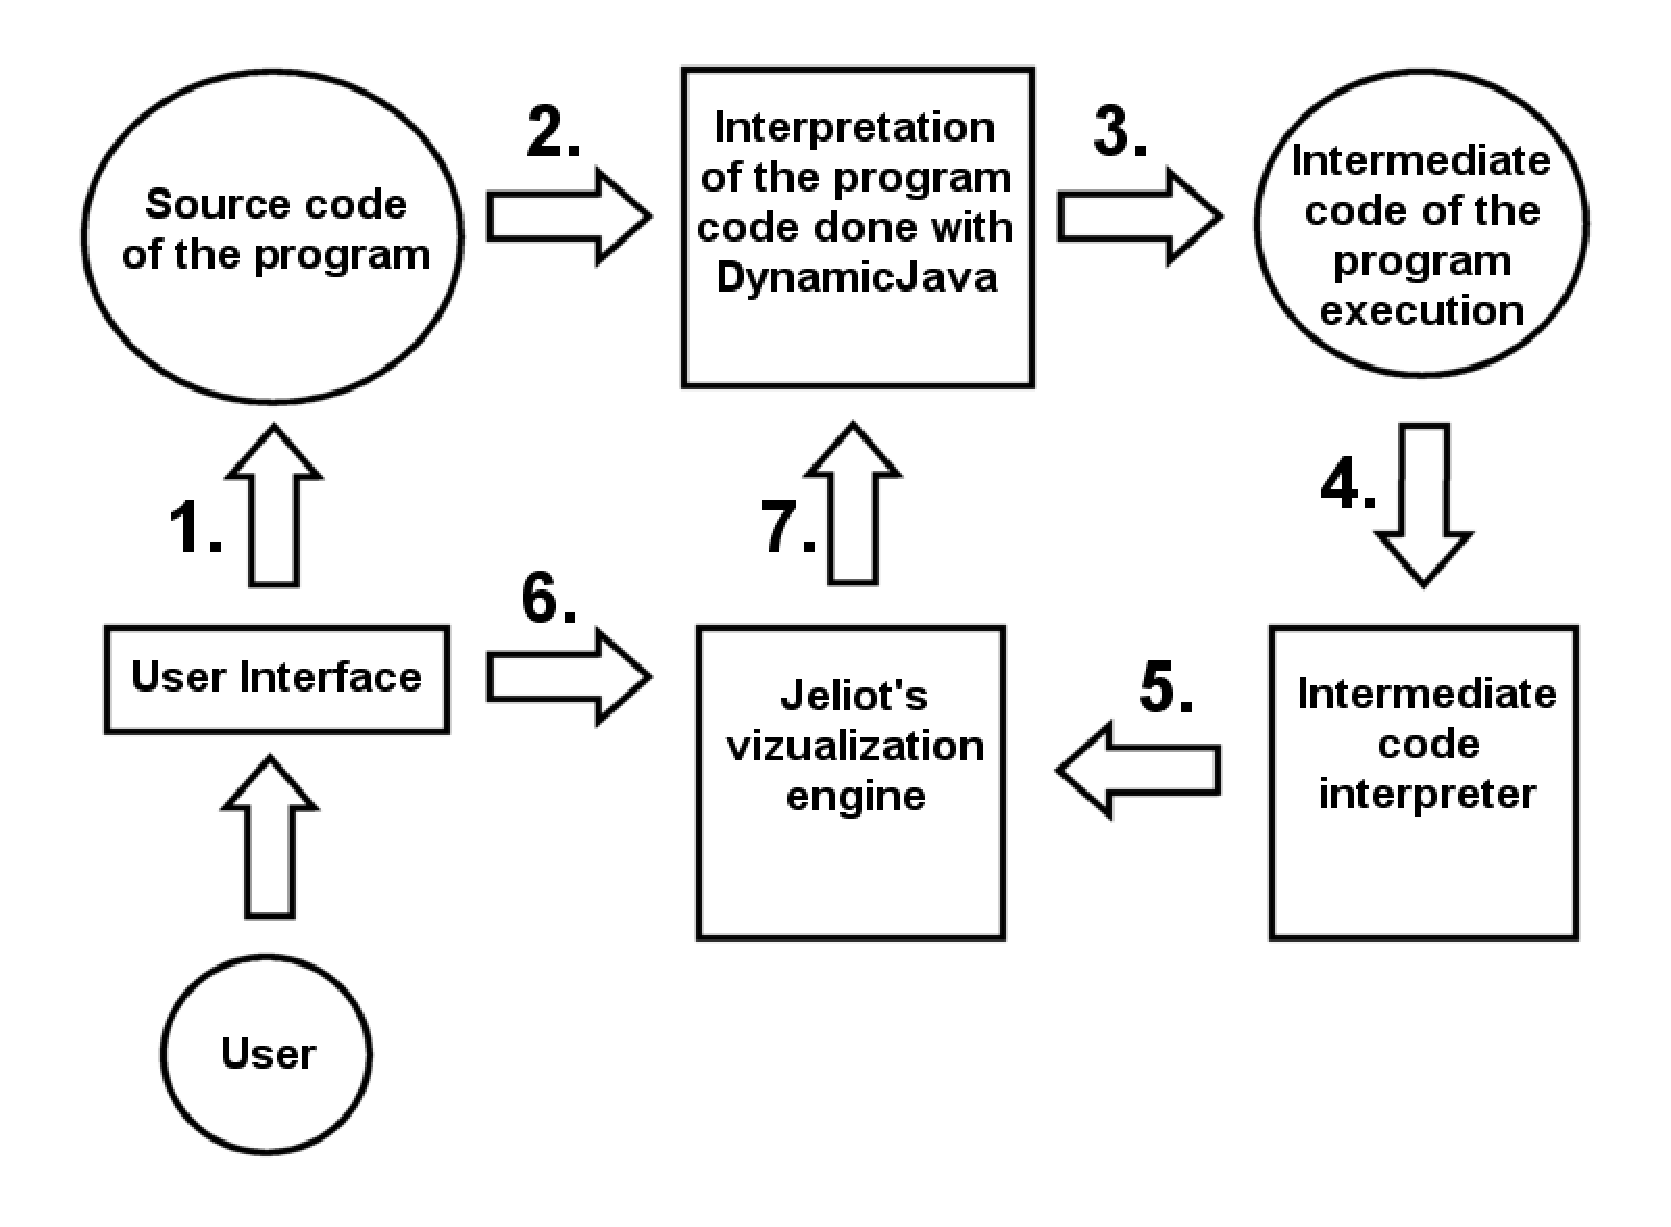
\includegraphics[height=10cm]{structure_of_jeliot_3.eps}
\caption{The functional structure of Jeliot~3.}
\label{fig:structure_of_jeliot_3}
\end{center}
\end{figure}

The functional structure of the Jeliot~3 is shown in the Figure~\ref{fig:structure_of_jeliot_3}.
A user interacts with the user interface and forms the source code of the program (1).
The source code is sent to the Java interpreter and the intermediate code is extracted (2 and 3).
The intermediate code is interpreted and the directions are given to the visualization engine (4 and 5).
A user can control the animation by playing, pausing, rewinding or playing step-by-step the animation (6).
Furthermore, the user can input data, for example, an integer or a string, to the program executed
by the interpreter (6 and 7).


%\newpage


\section{The Structure of \jel{} System}
\label{sec:The_Components_of_the_Jeliot_3_System}

We introduce here the different components of \jel{} systems. The system
contains several packages and here we explain those that are most crucial
in understanding the structure of \jel{}. Only package and classes related
to communication between visualization engine and \djava{} are introduced
in the chapter~\ref{sec:Communications_Model}.

The functional structure of the Jeliot~3 is shown in the
Figure~\ref{fig:structure_of_jeliot_3}. A user interacts with the user
interface and forms the source code of the program (1). The source code
is sent to the Java interpreter and the intermediate code is extracted
(2 and 3). The intermediate code is interpreted and the directions are
given to the visualization engine (4 and 5). A user can control the
animation by playing, pausing, rewinding or playing step-by-step the
animation through the user interface (6). Furthermore, the user can
input data, for example, an integer or a string, to the program
executed by the interpreter (6, 7 and 8).

\begin{figure}[htbp]
\begin{center}
\begin{picture}(400,250)

% BOXES, OVALS and CIRCLE
%--------------------------
%User group
\put(50,30){\circle{60}}
\put(20,0){\makebox(60,60){\f{User}}}
%User interface
\put(10,90){\framebox(80,20){\f{User interface}}}
%Source code
\put(50,200){\oval(80,50)}
\put(10,175){\makebox(80,50){\shortstack{\f{Source code}\\\f{of the program}}}}
%DJava
\put(160,160){\framebox(80,80){\shortstack{\f{Interpretation}\\\f{of the program}\\\f{code done by}\\\f{\djava{}}}}}
%Intermediate code
\put(350,200){\oval(80,70)}
\put(310,165){\makebox(80,70){\shortstack{\f{Intermediate}\\\f{code of the}\\\f{program}\\\f{execution}}}}
%Visualization engine
\put(160,60){\framebox(80,50){\shortstack{\f{Visualization}\\\f{engine}}}}
%Intermediate code Interpreter
\put(310,60){\framebox(80,50){\shortstack{\f{Intermediate}\\\f{code}\\\f{Interpreter}}}}
% VECTORS
%----------------------------
% 0. (user, user interface) (user interface, user)
\put(40,47){\vector(0,1){43}}
\put(60,90){\vector(0,-1){43}}
% 1. (user interface, source code)
\put(50,110){\vector(0,1){65}}
\put(50,110){\makebox(20,65){\f{1.}}}
% 2. (source code, djava)
\put(90,200){\vector(1,0){70}}
\put(90,200){\makebox(70,20){\f{2.}}}
% 3. (djava, intemediate code)
\put(240,200){\vector(1,0){70}}
\put(240,200){\makebox(70,20){\f{3.}}}
% 4. (intemediate code, intemediate code interpreter)
\put(350,165){\vector(0,-1){55}}
\put(350,110){\makebox(20,55){\f{4.}}}
% 5. (intemediate code interpreter, visualization engine)
\put(310,100){\vector(-1,0){70}}
\put(240,100){\makebox(70,20){\f{5.}}}
% 6. (user interface, visualization engine)
\put(90,100){\vector(1,0){70}}
\put(90,100){\makebox(70,20){\f{6.}}}
% 7. (intemediate code interpreter, visualization engine)
\put(240,80){\vector(1,0){70}}
\put(240,80){\makebox(70,20){\f{7.}}}
% 8. (visualization engine, Djava)
\put(310,110){\vector(-1,1){70}}
\put(260,130){\makebox(50,50){\f{8.}}}
\end{picture}
\caption{The functional structure of Jeliot~3.}
\label{fig:structure_of_jeliot_3}
\end{center}
\end{figure}

Different packages of \jel{}~3 are introduced in this section in
the same order as in the functional structure. In this way we
hope that all the components and their meaning becomes clearer.

\subsection{\jel{} Class}
\label{sec:Jeliot_Class}

Class \jel{} in the package \p{jeliot} is the main class of the program.
It combines the different components of the program together a deals with
some communicational issues. When the program is started the class creates
all the needed components and passes them as parameters to the user interface
classes. It mainly handles the communication between the user interface
(\p{jeliot.gui}) and the theater/animation engine (\p{jeliot.theatre}) classes.
In addition to that it also invokes the thread handling the interpretation
of the user program.

\subsection{User Interface}
\label{sec:User_Interface}

The user interface of Jeliot is located in the package \p{jeliot.gui}.
The structure of the user interface is shown in the
Figure~\ref{fig:jeliot3_UI_structure}. The main
class is \p{JeliotWindow} that extends \p{JFrame}. The frame is layed out
by \p{BorderLayout}. A split pane (\p{JSplitPane}) is added in the center and
a panel containing control panel (created in \p{JeliotWindow}) and output console
(\p{OutputConsole}) is added in the south (bottom) border.

In the split pane the left side is used by code editor (\p{CodeEditor}) or code viewer
(\p{CodeViewer}). Code editor is shown during editing of the program
and code viewer during the animation of the program. Both of the text components
have a line numbering component (\p{LineNumbers} on their row header. Moreover,
code editor consist of editing panel that has a few buttons to load, save and
edit the source code. The frame has also a menu bar that is constructed
partially in \p{CodeEditor} class and partilly in \p{JeliotWindow} class.

On the right hand side of the split pane a animation engine called
theater (\p{Theatre}) is normally shown. However, if any errors occur
during the compilation or run-time of the program they are shown
in the \p{Error viewer} (\p{ErrorViewer}) instead of theater.

\p{JeliotWindow} combines all the components in \p{jeliot.gui} package and
creates the user interface. It also deals with most of the events
happening during the {run-time} and delegates the commands forward to
the appropriate classes (e.g. \p{Jeliot} or \p{CodeEditor}). Other classes
in the \p{gui} package are related to one of the components introduced in the
previous paragraph. There are also three classes that are not currently in use
in \jel{}~3, namely \p{LoadJeliot}, \p{DraggableComponent} and \p{TheatrePopup}.

\begin{figure}[htbp]
\begin{center}
\begin{picture}(300,200)
%overall frame
\put(0,0){\framebox(300,200){\ }}
%Menu bar
\put(0,170){\framebox(100,30){\f{Menu bar}}}
%Code editor
\put(0,40){\framebox(100,130){\shortstack{\f{Code editor}\\\f{or}\\\f{Code viewer}}}}
%Theatre
\put(100,40){\framebox(200,160){\shortstack{\f{Animation frame (Theatre)}\\\f{or}\\\f{Error viewer}}}}
%Control panel
\put(0,0){\framebox(120,40){\f{Control panel}}}
%Output Console
\put(120,0){\framebox(180,40){\f{Output Console}}}
\end{picture}
\caption{The structure of user interface in Jeliot~3.}
\label{fig:jeliot3_UI_structure}
\end{center}
\end{figure}

\subsection{DynamicJava}
\label{sec:DynamicJava}

DynamicJava consists of 7 different packages, where only five
of them actually perform the interpretation: \p{classfile}, \p{classinfo},
\p{interpreter}, \p{parser} and \p{tree}. The other two (\p{util} and \p{gui}) are
used to help the debugging of DynamicJava and to provide a nicer
user interface to the interpreter. For example, the \p{displayVisitor},
included in the util package, provides a nice output from the syntax tree.

\begin{itemize}
\item \p{Classfile} contains all the classes for creating general purpose bytecode
classes. The most important class is ClassFile which is the heart
of the class creation process.

\item \p{Classinfo} contains all the classes and interfaces for using reflection
on Java or interpreted classes. This package is used during
the compilation of the classes.

\item \p{Interpreter} contains the classes for interpreting Java language statements.
This is the most important package. It contains the most important
visitors that will be explained later.

\item \p{Parser} provides the classes that compose the default parser for the
language. The parser itself is represented by the class \p{Parser}.
The parser is generated by JavaCC 1.0. It creates the nodes of the
tree to be traversed later by the interpreter visitors.

\item \p{Tree} provides classes and interfaces for producing an abstract syntax
tree. This package does not depend of any non standard java package.

The created tree consists of nodes, the main data structure used
in \djava{}. All nodes have common properties, the segment
of source code where that node refers. Subclasses of this node
are defined to address the unique properties of each different
Java (e.g. staments and constructions). For example a node for
any binary expression will also consist of the properties \p{LEFT\_EXRESSION}
and \p{RIGHT\_EXPRESSION}.

\end{itemize}

Figure \ref{fig:Packages_visitors_and_data_flow_in_DJava} explains the
main relationships between the packages, the visitors and the main data flow.

\begin{figure}[htbp]
\begin{center}
\begin{picture}(400,200)
\put(110,20){\framebox(270,130){\ }}
\put(220,20){\makebox(50,20){\f{Interpreter}}}

\put(0,50){
\put(0,15){\vector(1,0){40}}
\put(0,15){\makebox(40,20){\shortstack{\f{source}\\\f{code}}}}
\put(40,0){\framebox(50,30){\f{Parser}}}
\put(90,15){\vector(1,0){40}}
\put(90,15){\makebox(40,20){\f{tree}}}
\put(130,0){\dashbox{5}(55,30){\shortstack{\f{Name}\\\f{Visitor}}}}
\put(185,15){\vector(1,0){35}}
\put(180,15){\makebox(40,20){\f{tree}}}
\put(220,0){\dashbox{5}(55,30){\shortstack{\f{Type}\\\f{Checker}}}}
\put(275,15){\vector(1,0){35}}
\put(270,5){\makebox(40,20){\shortstack{\f{tree}\\\f{and}\\\f{class}}}}
\put(310,0){\dashbox{5}(55,30){\shortstack{\f{Evaluation}\\\f{Visitor}}}}
\put(365,15){\vector(1,0){35}}
\put(360,15){\makebox(40,20){\f{result}}}
}

\put(240,80){\vector(0,1){20}}\put(250,100){\vector(0,-1){20}}
\put(240,130){\vector(0,1){40}}\put(250,170){\vector(0,-1){40}}
\put(60,80){\vector(0,1){90}}\put(70,170){\vector(0,-1){90}}
\put(270,180){\vector(1,0){40}}\put(310,190){\vector(-1,0){40}}

\put(220,100){\dashbox{5}(55,30){\shortstack{\f{TreeClass-}\\\f{Compiler}}}}

\put(0,170){
\put(40,0){\framebox(50,30){{\f{Tree}}}}
\put(220,0){\framebox(50,30){{\f{ClassInfo}}}}
\put(310,0){\framebox(50,30){{\f{ClassFile}}}}
}

\end{picture}
\caption{Packages, visitors and data flow in \djava{}}
\label{fig:Packages_visitors_and_data_flow_in_DJava}
\end{center}
\end{figure}

As we can see in the image DynamicJava carries the source code
through three visitors: \p{NameVisitor}, \p{TypeChecker} and, finally,
\p{EvaluationVisitor}. We also see how \p{EvaluationVisitor} will receive
a class from \p{TypeChecker}, the reason of this behaviour will be explained
in the next paragraphs.

The NameVisitor is a tree visitor that resolves the ambiguity in identifiers
in a syntax tree. As declared, this visitor traverses the tree trying to find
out syntactical ambiguities.

The \p{TypeChecker} is a tree visitor that checks the typing rules and loads the
classes, fields and methods. This \p{TypeChecker} class is not only worried
about typing rules. When visiting a class declaration, it invokes
\p{TreeCompiler}, which compiles the class into Java bytecode. However, this
compiling process \textit{alters the class} and the formed \textit{bytecode
does not match the original source code} of the class.

The \p{EvaluationVisitor} is a tree visitor that evaluates each node of
a syntax tree. This visitor is the one that performs the evaluation and
execution of the program. It usually starts by invoking the main method
of the compiled class. We can easily observe how it traverses
the syntax tree and modifies \djava{} structures to store information
and thus we can interfere with its normal interpretation to extract
the information it produces while interpreting the source code.

\subsubsection{Tree package}
\label{sec:Tree_package}

The \p{Tree} package has a class for every different Java language
construct. These classes are organized also as a tree. The class
Node is the one that every other class inherits, directly or
indirectly. It defines only one thing, the location of the node in
the source code, both the file and the position inside it. Most of
the other classes also define properties that later are inherited
by more specific classes.

The tree organization is shown in the
Diagrams~\ref{fig:several_tree_classes},
\ref{fig:primary_expression_classes}, \ref{fig:statement_classes}
and \ref{fig:un_and_bin_exp_classes}. These figures do not depict
all the nodes. Especially those that do not add more information.

Figure~\ref{fig:several_tree_classes} shows the different kind of
declarations, initializers and types. Two main types are used by
\djava{}: Array type and and primitive types. String are not
considered as a different type as it is a class. It is Java that
supports it by normal String methods.

\begin{figure}[!htb]
\begin{center}
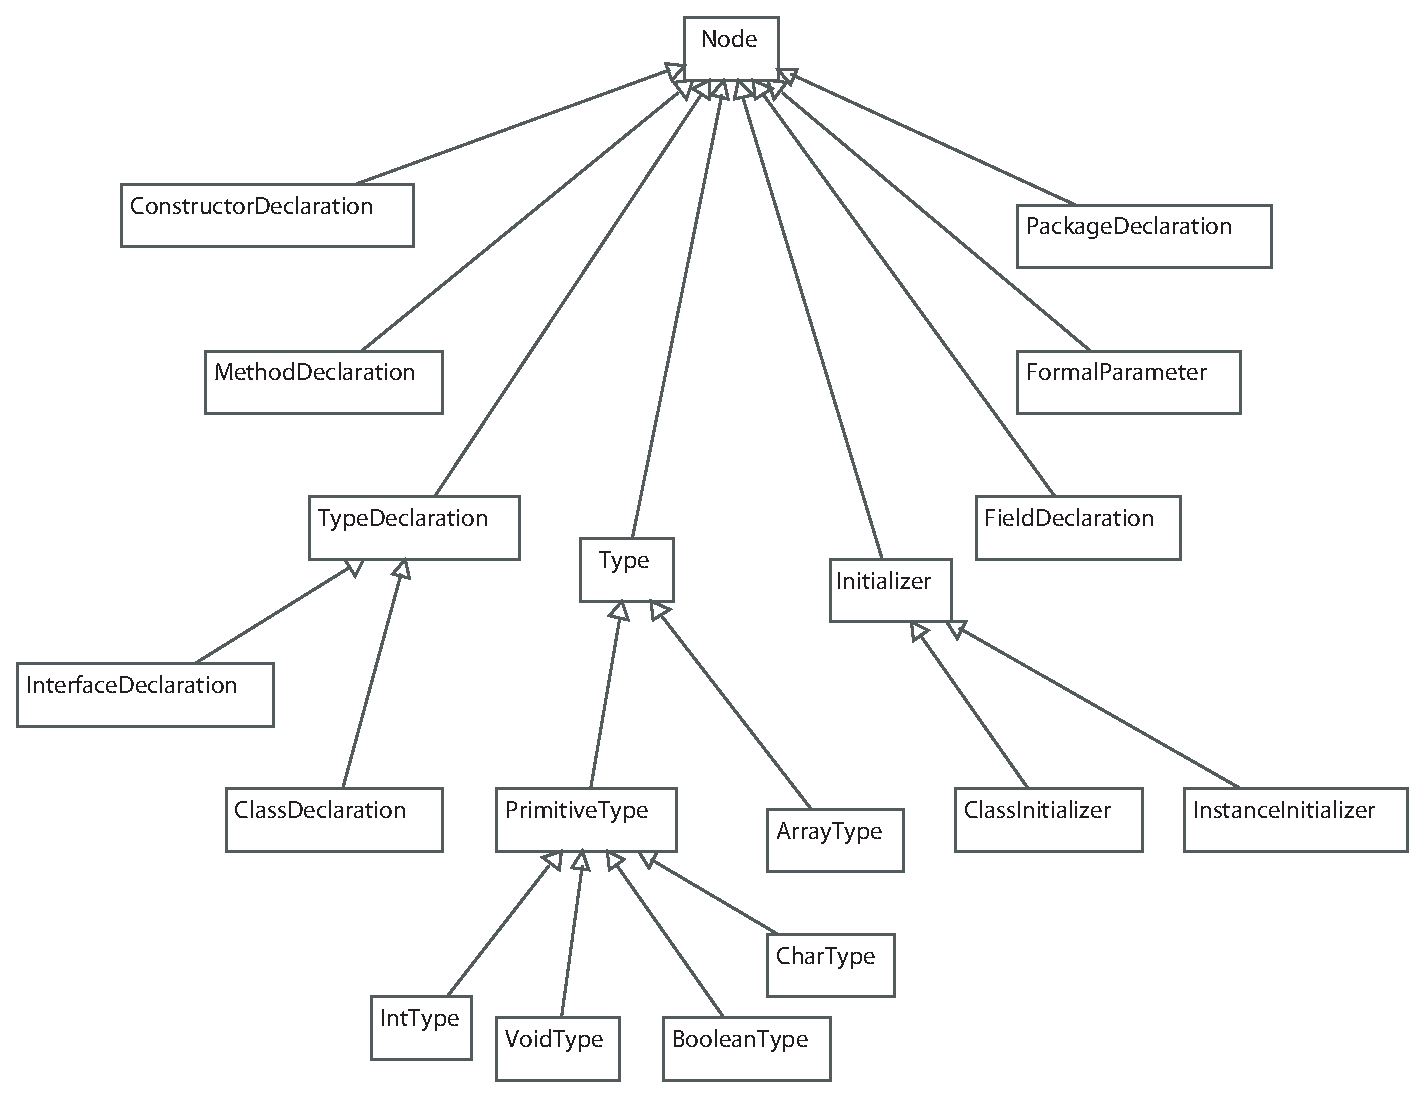
\includegraphics[width=\textwidth]{images/several.eps}
\caption{Several Tree classes. (Change the caption)}
\label{fig:several_tree_classes}
\end{center}
\end{figure}

Figure~\ref{fig:primary_expression_classes} shows the primary
expressions classes. Its super class, Expression, is also super
class for binary and unary expressions. All properties are defined
by Primary Expression subclasses. Some of those also implement
interfaces, even more than one. Interfaces are used by \djava{} to
know when certain conditions hold. Those that implement
\p{LeftHandSide} interface (\p{ArrayAccess}, \p{QualifiedName},
\p{FieldAccess}) are available to be the left hand side of an
assignment. Those that implement \p{ExpressionContainer} (\p{ObjectMethodCall},
\p{ReturnStatement}, \p{Constructor\-Invocation},
\p{ObjectFieldAccess}, \p{ArrayAccess}, \p{UnaryExpression}) are
those that need another expression to be completed. An array
access needs a qualified name where to look for the data, that
qualified name is the expression contained. The interface
\p{ExpressionStatement} is used only when \p{DynamicJava} parses
the source code to build up the \p{ForStatement} node.

\begin{figure}[!htb]
\begin{center}
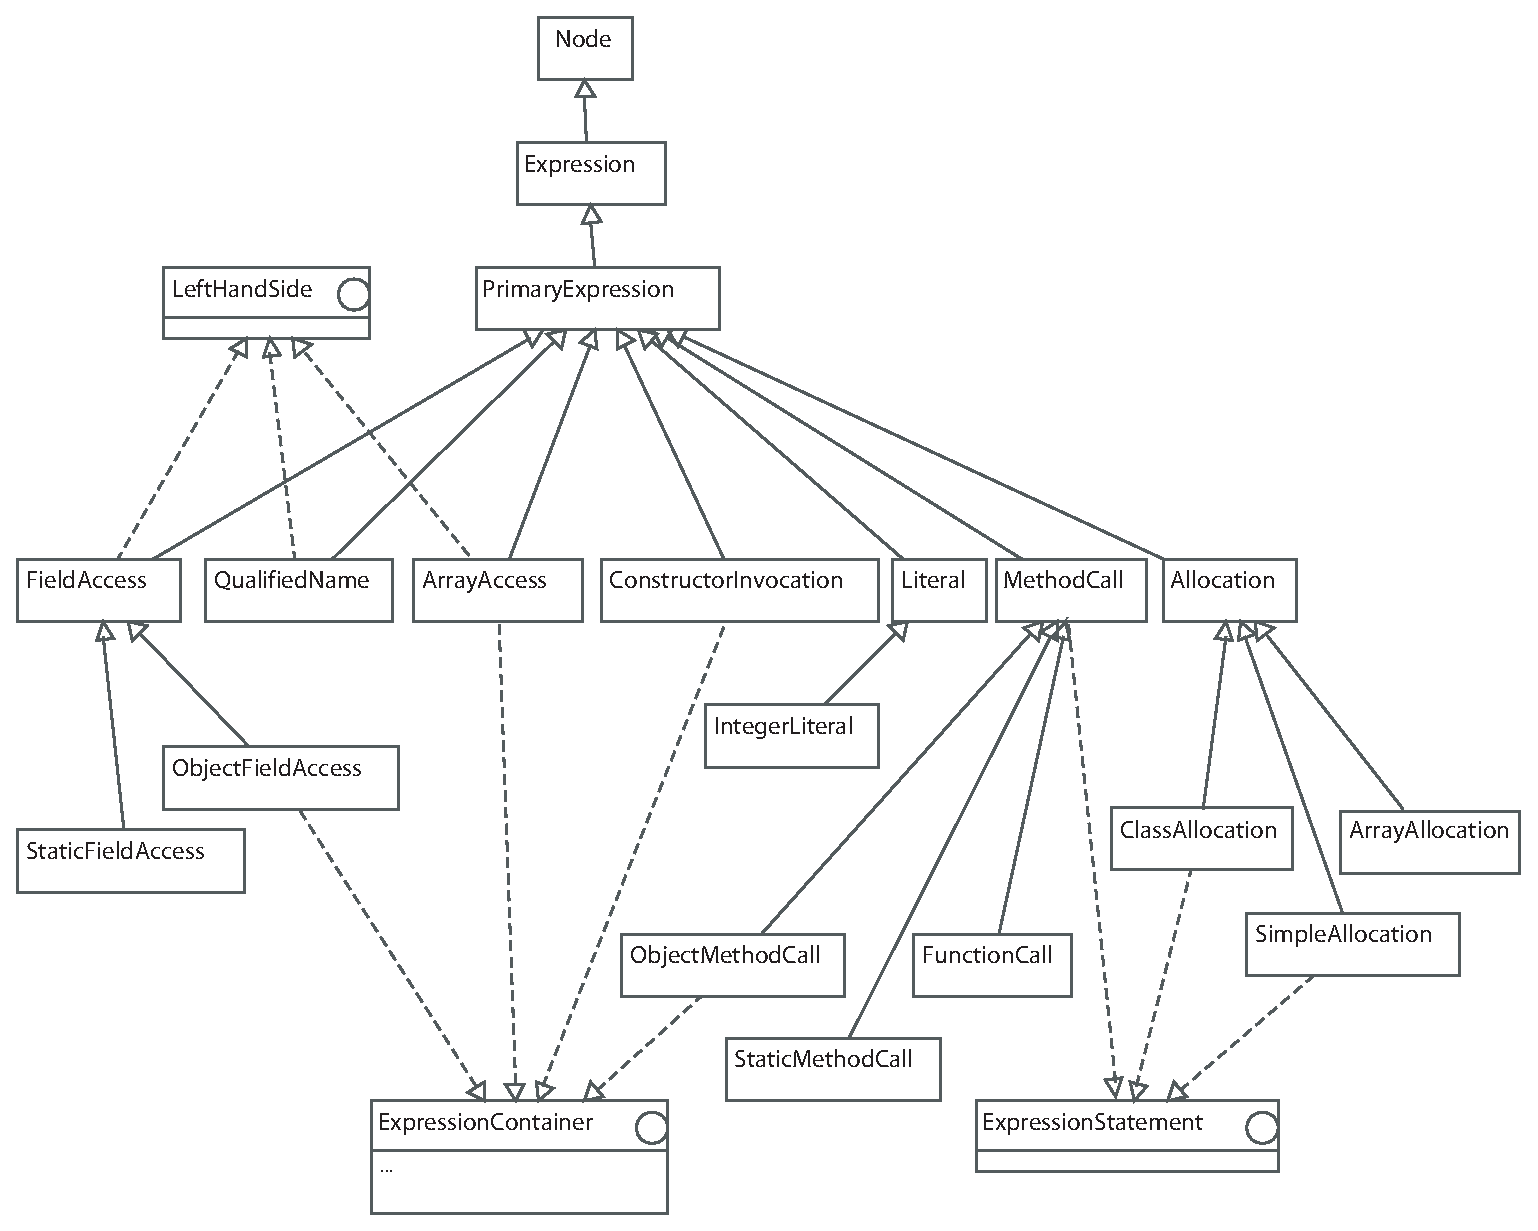
\includegraphics[width=\textwidth]{images/primaryexpressions.eps}
\caption{Primary expressions classes in \p{tree} package. (Change the caption)}
\label{fig:primary_expression_classes}
\end{center}
\end{figure}

Figure~\ref{fig:statement_classes} contains all the possible Java
statements. \p{ReturnStatement} is implementing
\p{ExpressionContainer} because it needs that interface when it is
returning an expression. \p{Do}, \p{While} and \p{For} statements
are implementing the \p{ContinueTarget} interface in order to
allow \p{ContinueStatements} inside of them.


\begin{figure}[!htb]
\begin{center}
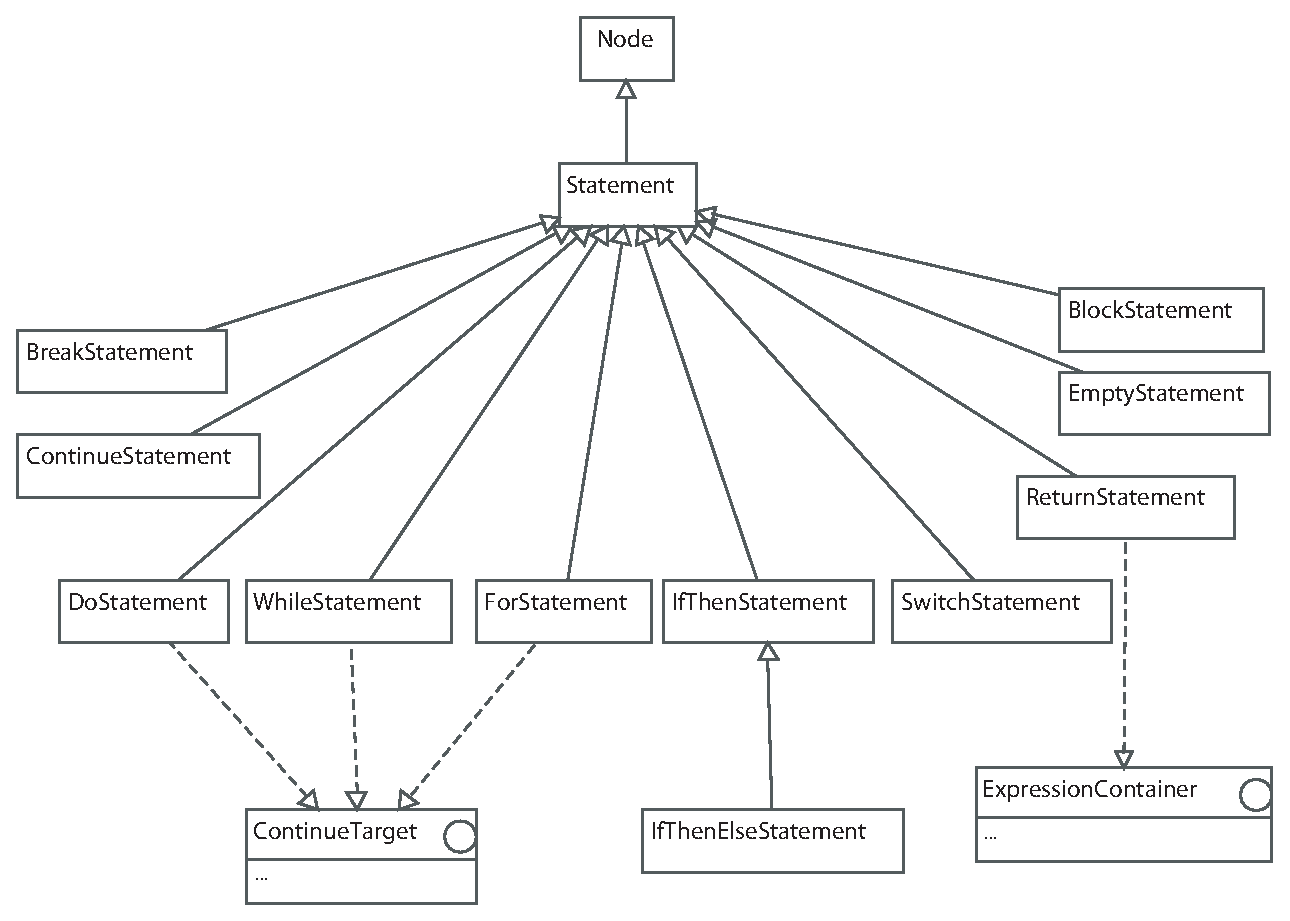
\includegraphics[width=\textwidth]{images/statements.eps}
\caption{Statement classes in \p{tree} package. (Change the caption)}
\label{fig:statement_classes}
\end{center}
\end{figure}

Figure~\ref{fig:un_and_bin_exp_classes} illustrates unary and
binary expressions. It only contains one as an example of each
their subclasses. So \p{AndExpression} also refers to
\p{OrExpression} and so on.

\begin{figure}[!htb]
\begin{center}
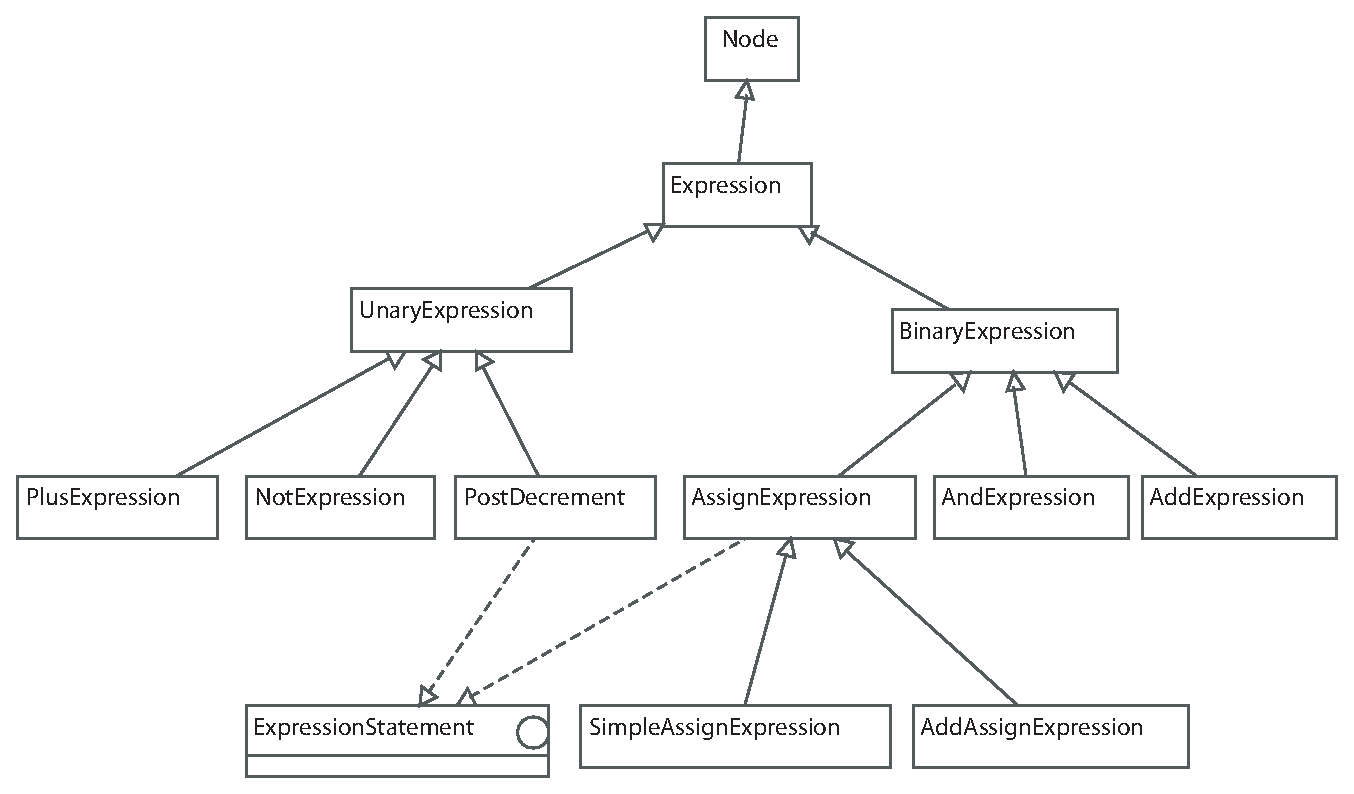
\includegraphics[width=\textwidth]{images/unary-bin-exps.eps}
\caption{Unary and binary expression classes in \p{tree} package. (Change the caption)}
\label{fig:un_and_bin_exp_classes}
\end{center}
\end{figure}

\subsection{Intermediate Code Interpreter}
\label{sec:Intermediate_Code_Interpreter}

The package \p{jeliot.ecode} includes the classes used by the intermediate
code interpreter. The class \p{Interpreter} contains the intermediate code
interpreter and the other classes  help the work with intermediate
code generation, interpretation and on the other aspects of the program execution.

The intermediate code is generated by the modified version of \djava{}. The code is
then written into a pipe that can be read by the interpreter. As the code is completely
machine written we know the form of the code and can interpret it easily. The intermediate
code is introduced in the section~\ref{sec:Intermediate_Code}. The code is read
line by line and it is tokenized with the agreed token in the class \p{Code} that contains
all the necessary constants for intermediate code generation. Then the first token tells what kind of statement is coming and how it should be processed. Then the rest of the statement is processed accordingly and a part of the animation is shown if necessary.

There are several important data structures in the \p{Interpreter} class:
\begin{description}
\item[\p{commands}] variable is a reference to a stack (\p{Stack}) that contains information about each read command. Command in this context tells, for instance, whether a operand of a binary operation is the left or right side of the operation.
\item[\p{exprs}] variable is a reference to a stack (\p{Stack}) containing the information about each read expression. The information consist of each expressions type (e.g. addition or subtraction operation), expression reference and the location in the code. It is used to
identify which operands (i.e. values or variables) belong to which operation.
\item[\p{values}] variable is a reference to a hash table (\p{Hashtable}) that contains the values of literals, variables and operations encountered during the execution. Each of the value is stored in a form of \p{Value} object (containing also the \p{Actor}) and the expression reference is used as a key for the hash table. These values are then used when an expression evaluation is animated.
\item[\p{variables}] variable is a reference to a hash table (\p{Hashtable})that contains the visited variables as instances of the \p{Variable} class.
\item[\p{instances}]
\item[\p{methodInvocation}]
\item[\p{postIncsDecs}]
\item[\p{currentClass}]
\item[\p{classes}]
\item[\p{currentMethodInvocation}]
\item[\p{objectCreation}]
\item[\p{returned, returnValue, returnActor, returnExpressionCounter}] are variables for handling the return value of a method.
\end{description}

Class \p{ECodeUtilities} is used by the interpreter to help type identification and
translating the intermediate code into the commands used in the visualization engine because they differ in some parts. It also handles some issues related to user input
and communication between \djava{} and the intermediate code interpreter.

\subsection{Language Constructs}
\label{sec:Language_package}

The classes of \p{jeliot.lang} package represent Java language constructs. They are mainly used to store and transfer the information about these language construct for the creation and handling of the corresponding \p{Actor}s (see section~\ref{sec:Actors}). The Figure~\ref{fig:language_constructs_and_actors} shows the class structure of the language construct classes and the corresponding \p{Actor}s that are used as attributes of the constructs. 

\begin{figure}[!htb]
\begin{center}
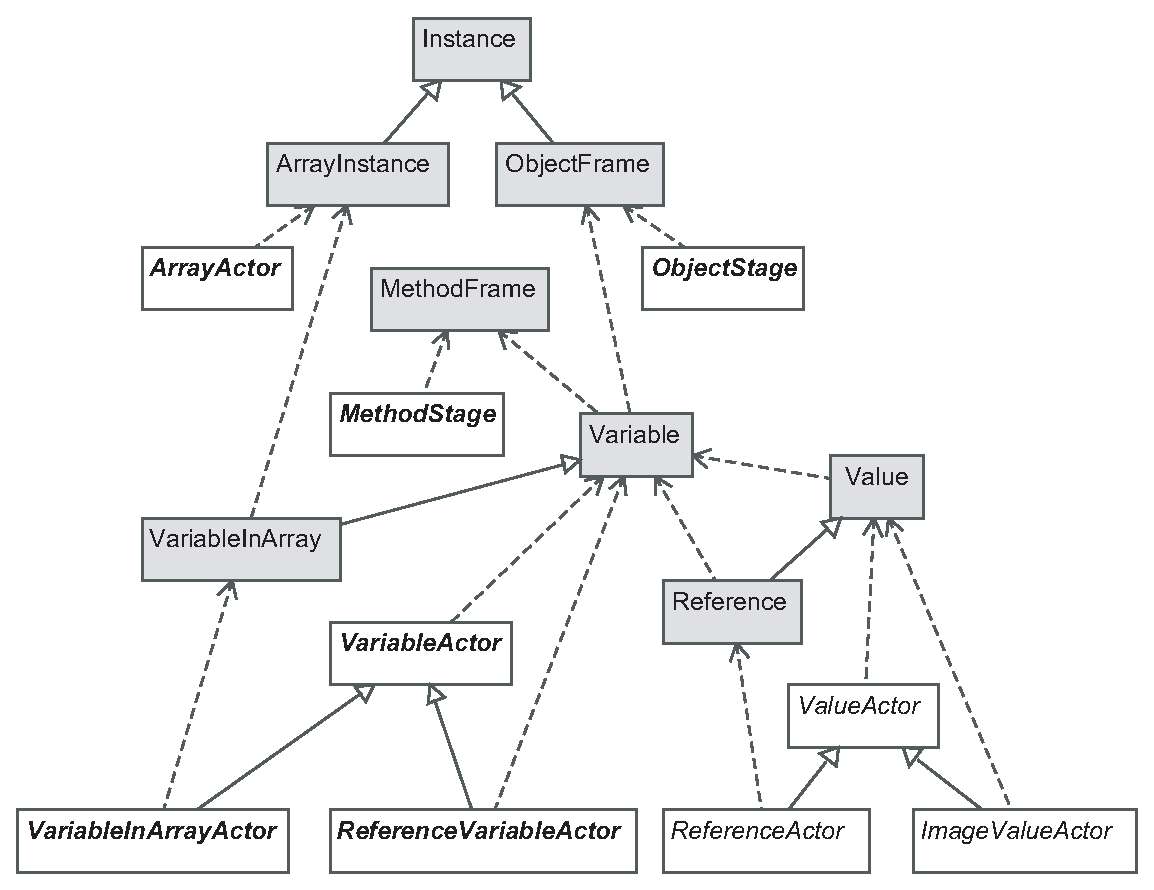
\includegraphics[width=\textwidth]{images/language_constructs_and_actors.eps}
\caption{The class hierarchy of the language constructs (gray boxes and solid lines) and the \p{Actor}s (white boxes and solid lines) and their usage relations to each other (dashed lines). \p{Actor}s (white boxes) implementing actor container are written in bold and italics and the other \p{Actor}s on just italics (see section~\ref{sec:Actors}).}
\label{fig:language_constructs_and_actors}
\end{center}
\end{figure}

\subsection{Visualization Engine}
\label{sec:Visualization_Engine}

The package \p{jeliot.theatre} contains classes that are used to form the animation.
We will here introduce the most important classes in the package and
tell the meaning of these classes. For rest of the classes see their
documented source codes.

\subsubsection{Theatre}

The \p{jeliot.theatre} package contains a class \p{Theatre} that extends \p{JComponent} class so that it can be entered inside the split pane in the user interface. It is the
canvas for the animation and all the actors are drawn on it.

See Figure~\ref{fig:jeliot3_theatre_structure}.

\begin{figure}[htbp]
\begin{center}
\begin{picture}(250,200)
%Overall frame
\put(0,0){\framebox(250,200){{\f{\bf{Theatre}}}}}
%Method frame area
\put(10,100){\dashbox{5}(80,90){\shortstack{\f{Method}\\\f{Stage}\\\f{Area}}}}
%Constant box
\put(10,10){\dashbox{5}(60,30){\shortstack{\f{Constant}\\\f{Box}}}}
%Instance Area
\put(80,10){\dashbox{5}(160,80){\shortstack{\f{Instance}\\\f{Area}}}}
%Expression Evaluation Area
\put(100,110){\dashbox{5}(140,80){\shortstack{\f{Expression}\\\f{Evaluation}\\\f{Area}\\\f{(Scratch)}}}}
\end{picture}
\caption{The structure of the animation frame (theatre) in Jeliot~3.}
\label{fig:jeliot3_theatre_structure}
\end{center}
\end{figure}

\subsubsection{Director class}

\p{Director} has a methods for different kind of operations during the
animation of the program (e.g. binary expression, unary expression,
object creation and method call). These methods are called by the intermediate code
interpreter (\p{ECodeInterpreter}). In each of the methods are given parameters
that the method needs for the operation.

Normally, first the method creates actors through \p{ActorFactory}
or uses existing actors. \p{Animation}s are created through \p{Actor}s' methods
(e.g. \p{appear} or \p{fly}). Created animations are given to
\p{AnimationEngine} to be run.Actors can be also added to other
\p{ActorContainer}s (e.g. \p{Theatre}, \p{VariableActor} or
\p{MethodStage}).

\subsubsection{Actor classes}
\label{sec:Actors}

See Figure~\ref{fig:class_hierarchy_of_Actor_class_small}.

\begin{figure}[!htb]
\begin{center}
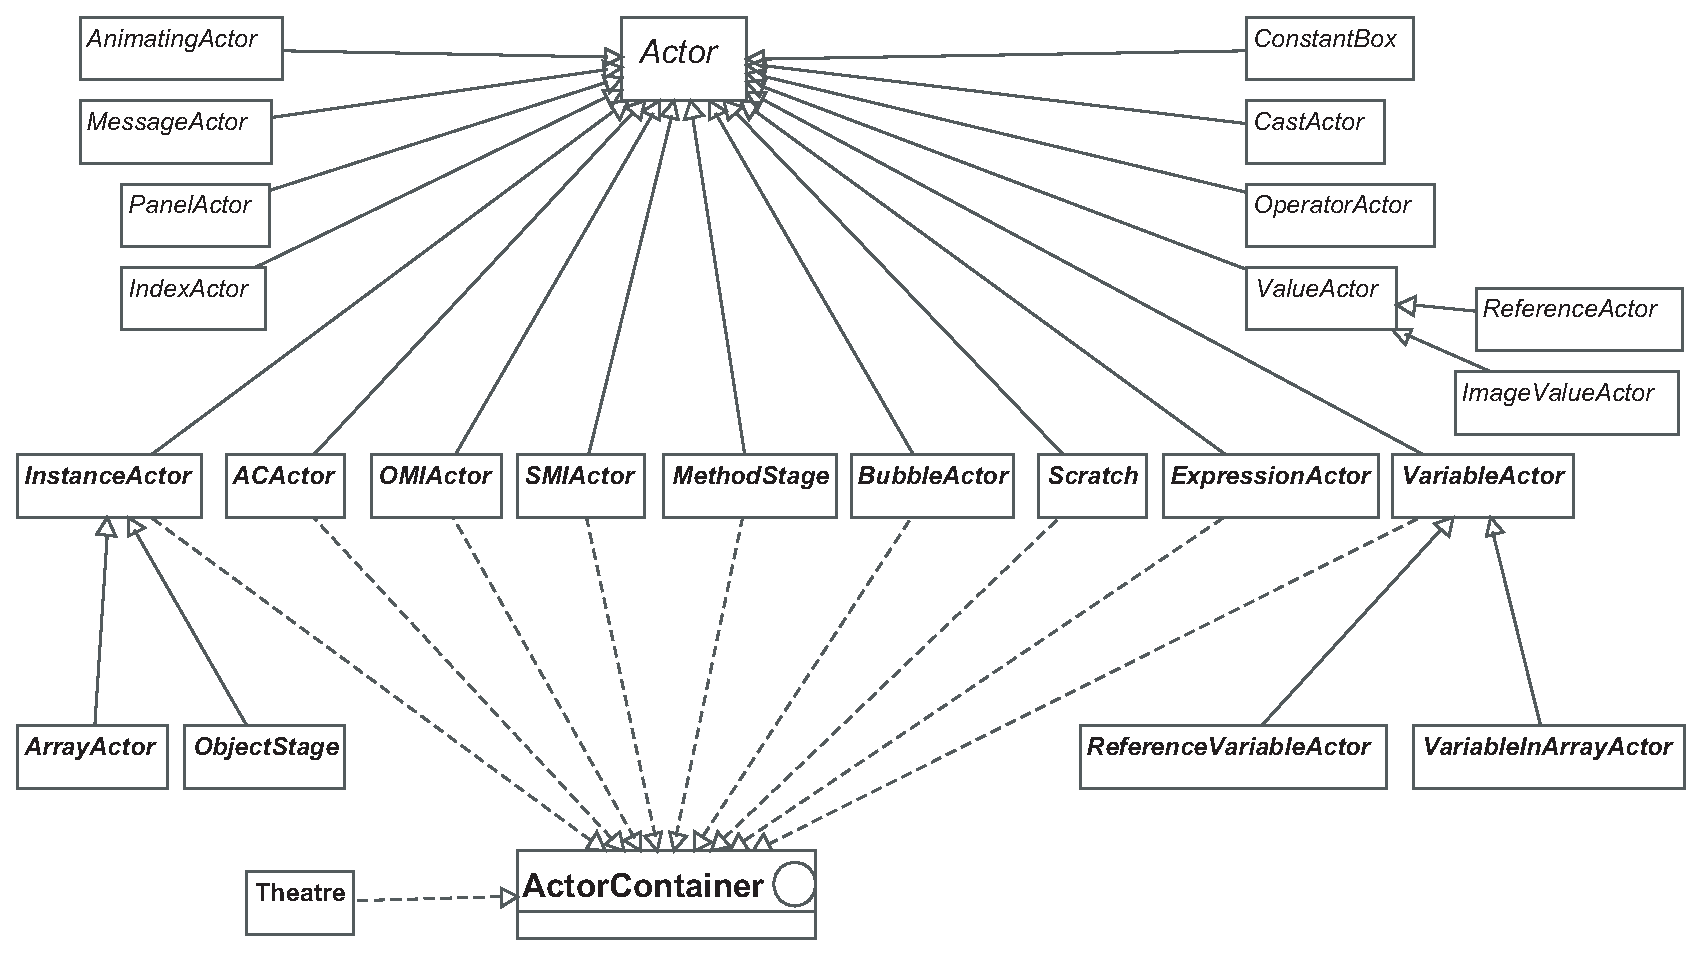
\includegraphics[width=\textwidth]{images/jeliot_actor_class_small.eps}
\caption{The class hierarchy of \p{Actor} class and \p{ActorContainer} interface.}
\label{fig:class_hierarchy_of_Actor_class_small}
\end{center}
\end{figure}

\subsubsection{ActorContainer interface}

See the Figure~\ref{fig:actors_and_actorcontainers}.

\begin{figure}[!htb]
\begin{center}
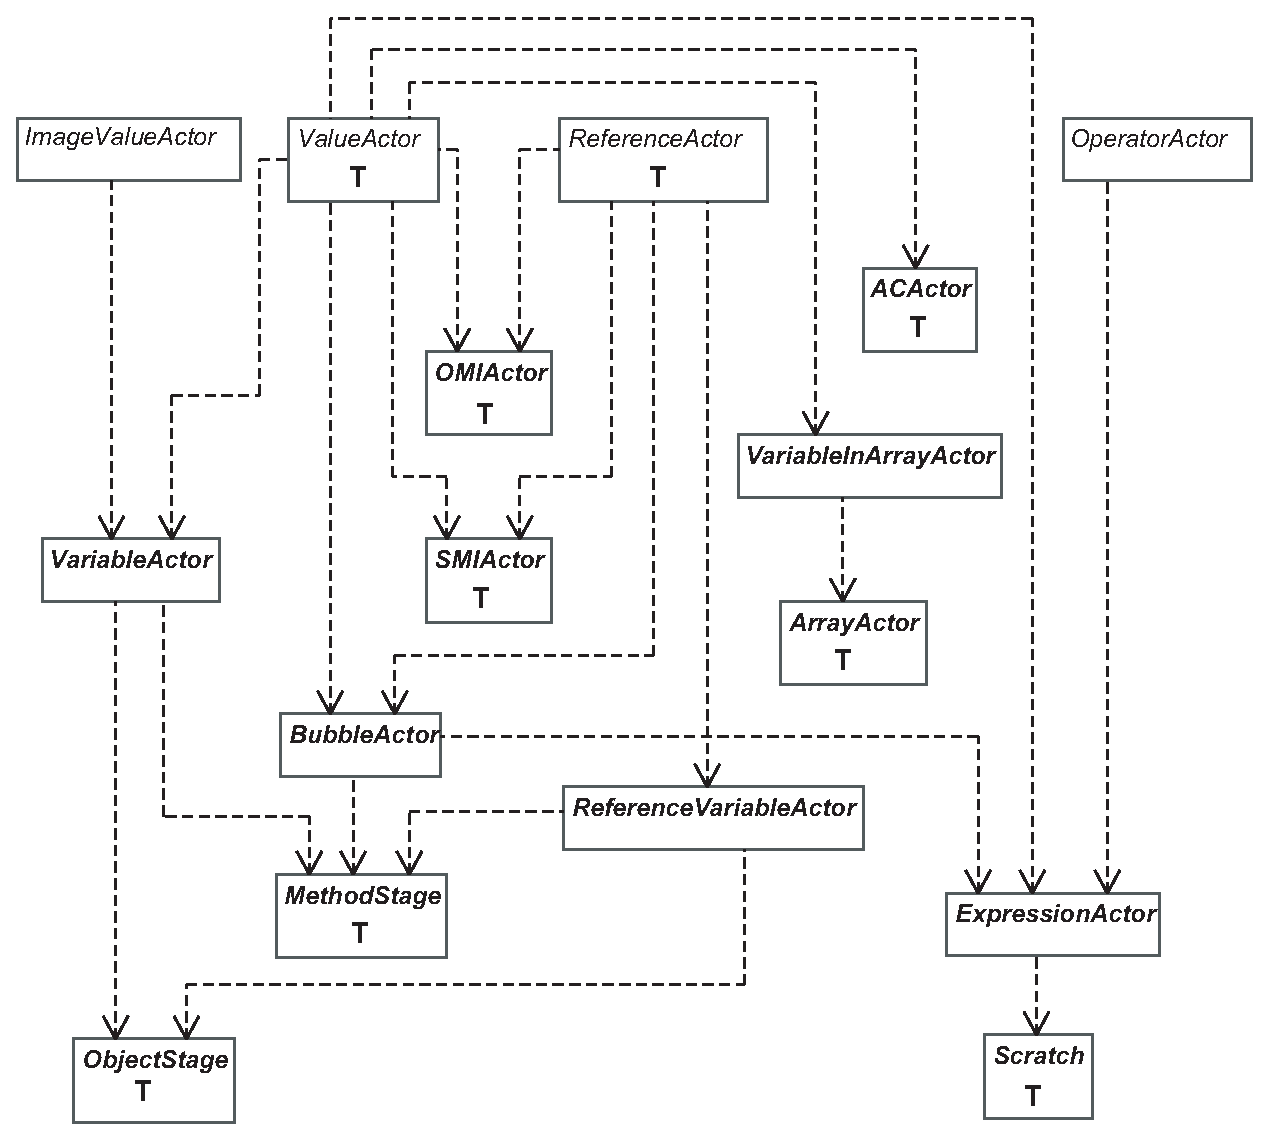
\includegraphics[width=10cm]{images/actorcontainers_and_actors.eps}
\caption{The inclusion relations between \p{Actor}s and \p{Actor}s implementing \p{ActorContainer} interface.}
\label{fig:actors_and_actorcontainers}
\end{center}
\end{figure}

\subsubsection{Animation class}

See the Figure~\ref{fig:jeliot3_animation_engine}.

\subsubsection{AnimationEngine class}

See the Figure~\ref{fig:jeliot3_animation_engine}.

\subsubsection{Theatre class}

See the Figure~\ref{fig:theatre_and_actorcontainers}.

\begin{figure}[!htb]
\begin{center}
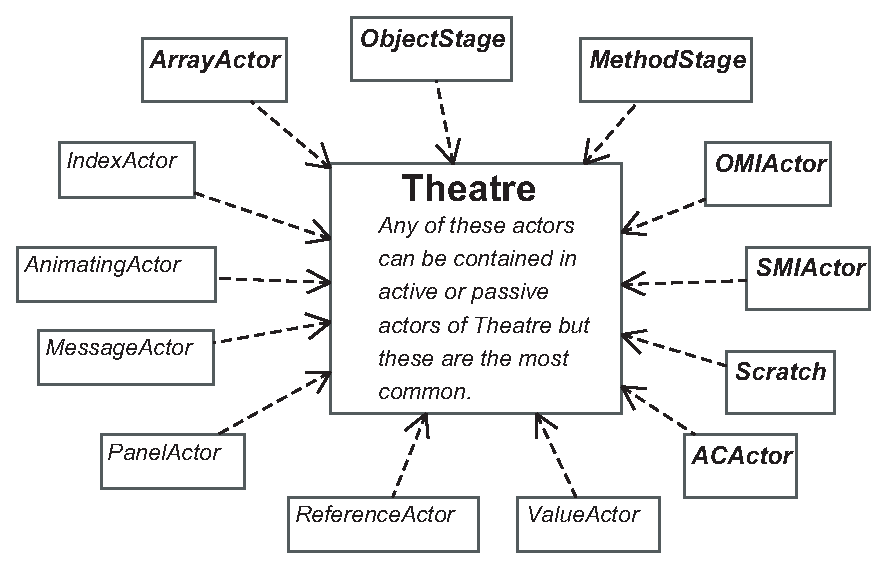
\includegraphics[width=10cm]{images/theatre_and_actors.eps}
\caption{The \p{Actor}s that are commonly included in the passive (\p{pasAct}) and active (\p{actAct}) \p{Actor}s.}
\label{fig:theatre_and_actorcontainers}
\end{center}
\end{figure}


\begin{figure}[!htb]
\begin{center}
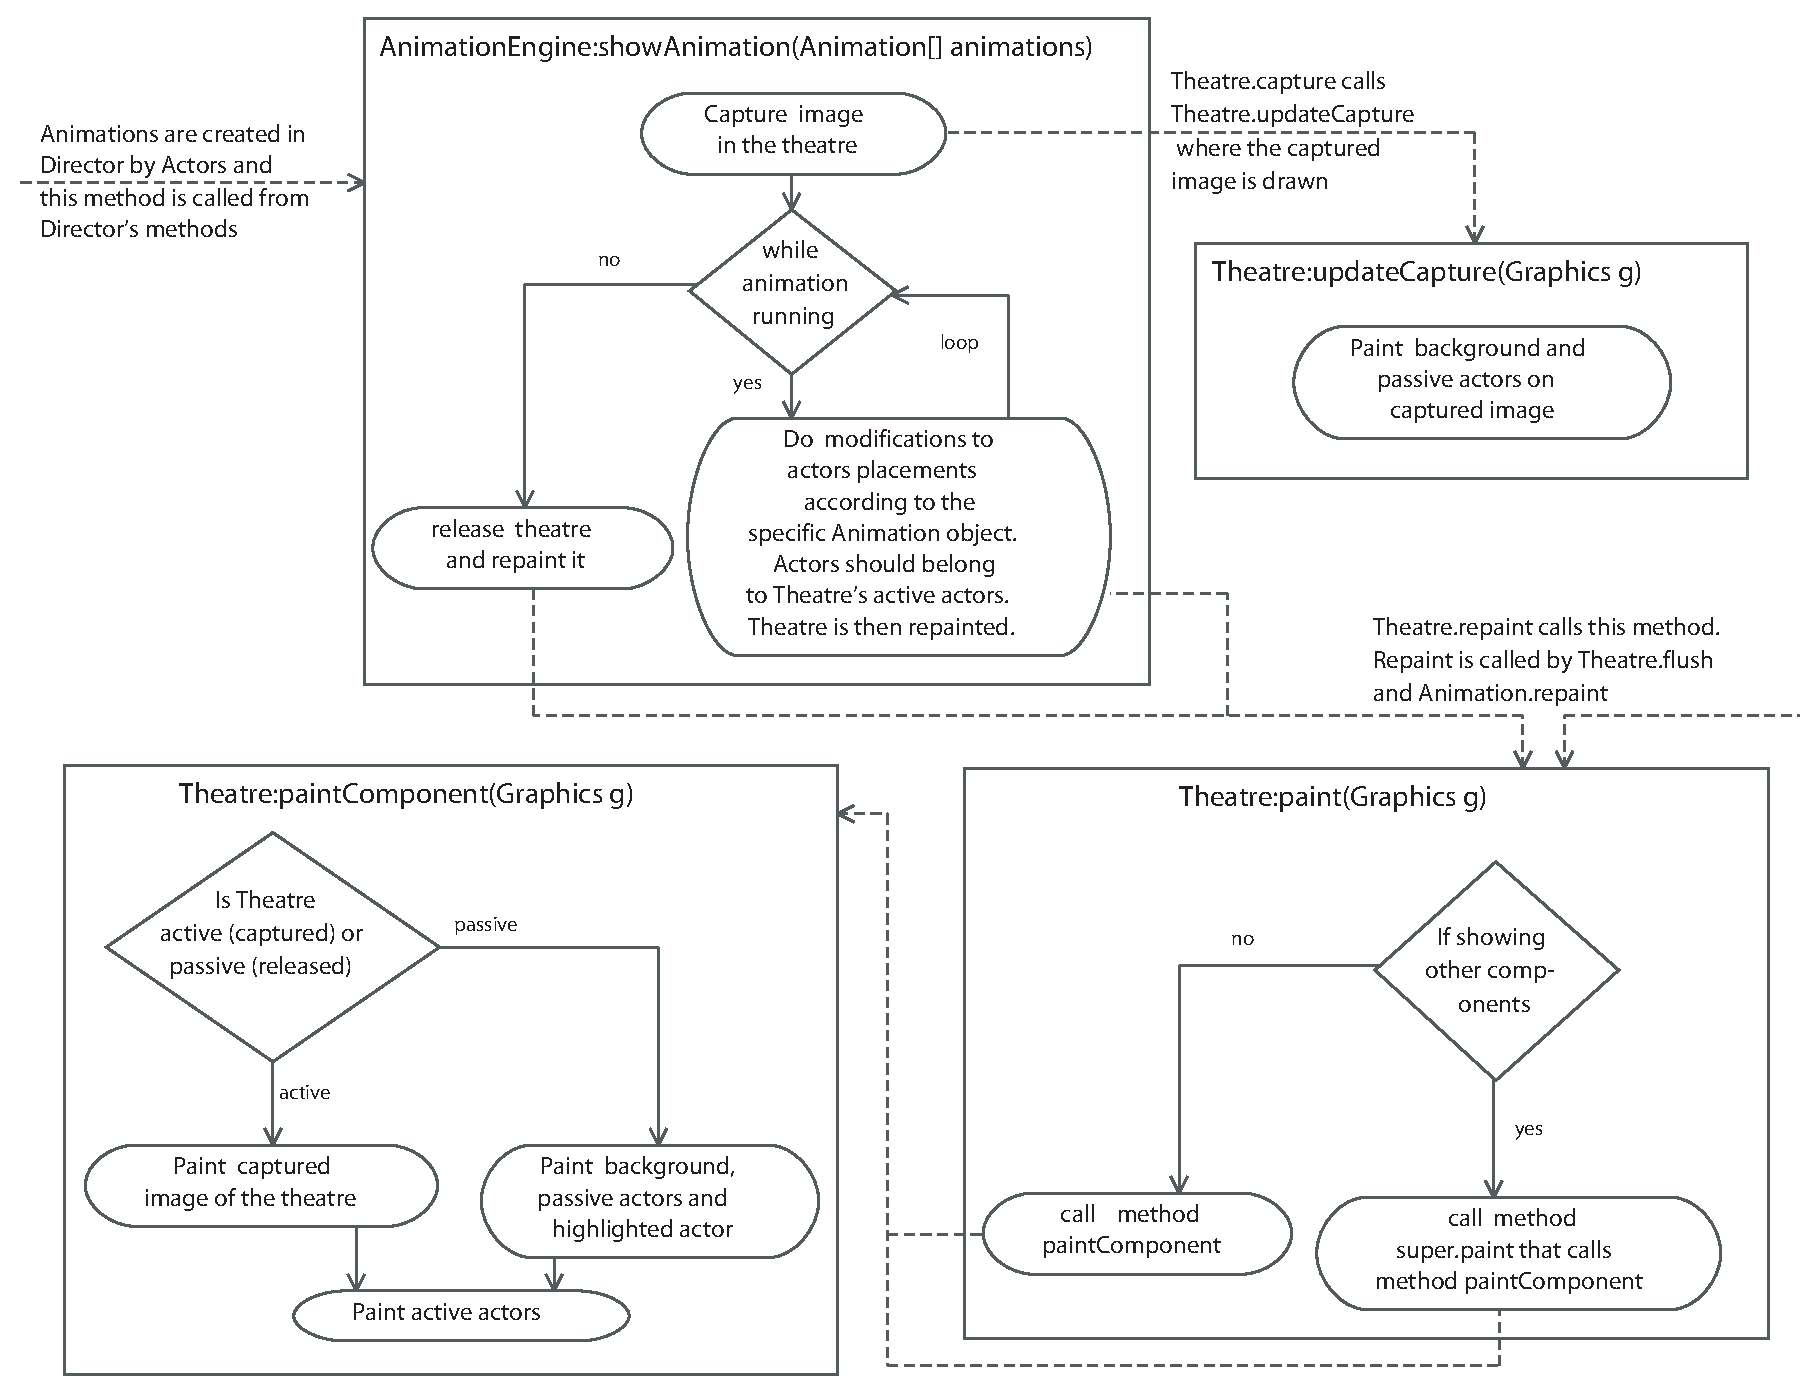
\includegraphics[width=\textwidth]{images/jeliot_animation_engine3.eps}
\caption{The structure of the animation engine in \jel{}.}
\label{fig:jeliot3_animation_engine}
\end{center}
\end{figure}

\subsubsection{TheatreManager class}


\subsubsection{ActorFactory class}

\newpage


\section{Communication Model}
\label{sec:Communications_Model}

{\bf Communication model here. Work for Andr{\'{e}}s}


\newpage


\section{Intermediate Code (M-Code)}
\label{sec:Intermediate_Code}

A new language was to be designed in order to express the
information extracted from the source code interpretation and pass
it to a new visualization interpreter. This interpreter will parse
these instructions (m-code sentences) and give the ``script'' of
the animation or ``play'' to \p{Director}, which organizes the
actors on the display. These cinematographic metaphors come from
the previous versions of \jel{}. \p{Director} stands for the
component that manages the different pieces of information
(actors) on the screen.

The m-code syntax is rather simple. While the inner representations
of the m-code commands are numbers, Java constants are used to
refer to them. The usual m-code sentence will consist of:

\begin{description}
\item[Expression/Statement code] A shortcut for every Java
statement or expression is used: e.g. AE stands for Add
Expression. The names chosen are closely related to the ones used
in \djava{}. \item[Reference] Every Expression/Statement sentence
is identified by a number. This way nested statements and
expressions can be formed up from previous {m-code} sentences.
\item[Related References] Most of the {m-code} sentences refer to
previous m-code sentences. One Add Expression will refer to the
references of both sides of expression. Flow-control statements
will refer to a condition expression, and so on. \item[Value] Most
sentences will return the value resulting from the executing of an
expression. If it is a flow control statement it will return a
boolean value indicating the result of the condition. \item[Type]
Every expression that has a result must specify its type.
\item[Location] This contains the location of the expression in
the original source code file.
\end{description}

Some auxiliary {m-code} commands have been defined to simplify m-code
interpretation, especially when referring to assignments and binary expression:
\begin{description}
\item[BEGIN] Indicates beginning of an assignment or expression.
It encapsulates nested expressions, literals or qualified names.
\item[LEFT] Indicates beginning of the left hand side of an expression.
\item[RIGHT] Indicates beginning of the right hand side of an expression.
\item[TO] Indicates the beginning of the assignment destination.
\item[END]  States the end of the current program execution.
\end{description}

One typical assignment like \p{a=b+1}; is coded as follows:
\begin{verbatim}
Begin|Assignment|1|1,1,1,10
Begin|AddExpression|2|1,5,1,10
Left|3
QualifiedName|3|b|1|int
Right|4
Literal|4|1|int|1,9,1,10
AddExpression|2|3|4|2|int|1,1,1,10
To|5
QualifiedName|5|a|UnknownValue|int
Assignment|1|2|5|2|int|1,1,1,10
\end{verbatim}

In this example we find two new commands \p{QUALIFIED NAME},
which refers to variables previously declared and \p{LITERAL} which states
for literal values, as numbers, characters or strings.

For a complete listing of commands and their descriptions see the
Intermediate Language Specifications document. (reference)

\subsection{M-code production}

\subsubsection{Evaluation Visitor}

As previously noted, \p{EvaluationVisitor} was the main class that
needed to be modified. In the next subsections, we will describe
how {m-code} is produced for certain subsets of Java expressions
and statements:

{\bf{Static Method Call}}

The visitor method \p{StaticMethodCall} is the entry point to the
evaluation visitor. It is the method called when invoking the main
method of a class from \p{TreeInterpreter}.

Here is where I/O management takes place. I/O facilities were to
be built-in in \djava{}, as they require special treatment in the
\jel{} side. We have chosen to keep on using the I/O library
provided by \jel{}~2000; nevertheless this can be changed by doing
some simple changes in \p{EvaluationVisitor}. So, to obtain the
I/O method calls, we first ask for the declaring class when
visiting a static method call [\p{public Object
visit(StaticMethodCall node)}],

\begin{itemize}
\item If it is an \p{Input} class we ask the \p{{m-code}
interpreter} to provide the information requested by ways of one
pipe that communicates with both sides. We discriminate the type
by the method name. Every input method has an equivalent in
\p{MCodeUtilities}, where the value is actually read from the
pipe. An m-code command named \p{INPUT} has been defined to
request data of a given type from the \p{Director}. \item If it is
an \p{Output} class then the only method currently available is
\p{println}. \djava{} visits the argument and sends the resulting
string to the \p{{m-code} interpreter} with the command
\p{OUTPUT}.
\end{itemize}

After that a stack is maintained by \p{StaticMethodCall} and
\p{ReturnStatement} visitors to manage multiple method calls (e.g.
\p{return object.method()}). A reference number is pushed into the
stack in every method call.

Later, the argument types are processed and m-code is produced to
inform \p{m-code interpreter} of these types. Finally \djava{}
will invoke the method with all the information. When the
invocation ends a special statement is produced to indicate the
end of static method call (\p{SMCC}).

However, when a static method call refers to a foreign method
(no source code is provided for it), the normal invocation will only
return the value, if it is not a void method. But to visualize the
call properly we need to simulate the parameters passing and the
method declaration m-code statements. Moreover, the value returned
must be inside a return m-code statement, again for visualization
purposes, so it is simulated too.

{\bf{Return Statement}}

A return statement can contain a value to return or nothing at all
(a void method or function). If there is something to be, returned
a \p{BEGIN} statement is produced before visiting the expression
to be returned. Otherwise a simple return statement is produced
with the special constant \p{Code.NO\_REFERENCE}, so \jel{}
interpreter will not look for an expression.

A stack is maintained by the \p{StaticMethodCall} and
\p{ReturnStatement} methods to manage recursive method calls (e.g.
\p{return object.method()}). A reference number is pushed onto the
stack in every method call. The return statement will pick it up
from the top of the stack and that will identify the return
statement.

{\bf{Simple Assign Expression}}

A \p{BEGIN} statement is produced indicating the beginning of a
new assignment. Then the right expression is visited and thus it
produces its own m-code. A special statement \p{TO} is produced
pointing the beginning of the left expression, where the value
obtained interpreting the right expression will be stored. This
left expression was not visited in the original \djava{}, as
it is not needed to modify the context. However we need to visualize
that expression, so an "artificial" visit was added. An \p{evaluating}
flag is set to show that it is an "artificial" visit. Finally we
produce the assign code with references to both expressions.

{\bf{Qualified Name}}

Qualified Names are the names already declared (e.g. variable
names and any other identifier) and they are used in expressions.
Its visitor was modified to take into account the \p{evaluating}
flag. The reason having two different behaviors is that \djava{}
throws an \p{ExecutionError} when visiting an uninitialized
qualified name. That occurs when an assignment method (as
\p{SimpleAssignExpression}) visits its left hand side for
visualization purposes before it has a value. When the
\p{evaluating} flag is false, \djava{} invokes the \p{display}
method to avoid unnecessary exceptions. However, both methods
(\p{visit} and \p{display}) produce the same m-code.

{\bf{Variable Declaration}}

Variable declaration does not cause large modifications to
original source code. Only if an initialization expression is
found, we have to modify the normal process to visualize the
initialization. This is done by simulating an assignment after the
variable is declared.

{\bf{Flow Control Statements}}

All flow control statements work similarly. Here, we will explain
how a \p{while} statement produces its m-code. Other statements
work in a similar way.

Firsts of all, the \p{WhileStatement} node keeps the reference to
the condition that will be visited and will determine whether to
enter or not the body of the statement. If the condition holds the
visitor produces a \p{WHILE} statement with \p{TRUE} as a value.
Then the body is evaluated, producing its own m-code.

Break or continue visitors throw exceptions to be caught by the flow
control statements. When they are caught their corresponding m-code
statement is produced. This statement reflects where the break or
continue has happened (\p{WHILE}, \p{FOR}, \p{DO} and \p{SWITCH} expression)

{\bf{Boolean and Bitwise Unary Expressions}}

This group contains the not (\p{!}) and complement (\p{\~})
operators. There are two different possibilities. On the one hand
the expression can be constant and not evaluation is performed by
\djava{}, so the generation of m-code is straightforward. However,
as there is no expression to be referred, there is no node
containing that constant, only a value is returned.
\p{Code.NO\_REFERENCE} is used to indicate this fact to the
interpreter. On the other hand, when there is an expression to
negate, a \p{BEGIN} statement is produced before the expression to
be negated is visited. Finally the unary statement is produced
returning the value and referring to the expression it affects.

{\bf{Unary arithmetic expressions}}

This group contains increments and decrements (\p{++}, \p{---}).
No special modifications were carried out in these visitors. They
just generate a \p{BEGIN} statement and their own statement
(\p{PIE}, \p{PDE}, \p{PRIE}, \p{PRDE}), that returns the modified
value and the type.

{\bf{Binary Expressions}}

This group comprises all boolean, bitwise and arithmetic binary
operators. As usual, a \p{BEGIN} statement is produced,
anticipating what the operator will be. Then both sides of the
expression are visited and their values are collected. Before each
of these two visits, there is one special m-code statement: a
\p{LEFT} statement, for the left side, and a \p{RIGHT} statement
for the right side. Finally the binary statement is generated
referring both sides and the value resulting of applying the
operator to both sides of the expression.

{\bf{Compound Assignment Expressions}}

This group contains all bitwise and arithmetic compound assignments.
Compound operators are for example \p{+=}, \p{-=}, \p{*=} and \p{/=}. The visitors of
these compound assignments have been modified to produce m-code that
decomposes the compound assignment into a simple assignment and a binary
operation. For example \p{a+=3-b} will be interpreted as \p{a=a+(-b)}.

Then, the code of the visitors is just a composition of an
assignment and a binary expression as its right hand side. This
binary expression has as its sides the same ones as the compound
assignment. As a result, two fake or artificial visits are done to
the left hand side of the compound assignment.

\subsubsection{Tree Interpreter}

This class contains methods to interpret the constructs of the language.
This class is the one called from Jeliot to start interpreting a program
or a single method. There are two main methods that have been modified.

{\bf{interpret(Reader r, String fname)}}

This method receives the source code and invokes the three
visitors of \djava{}: \p{NameVisitor}, \p{TypeCheker} and
\p{EvaluationVisitor}. This method catches the execution and
parsing errors and generates m-code to notify Jeliot of the
possible lexical, syntax or semantic errors that are found during
the interpretation.

{\bf{interpretMethod(Class c, MethodDescriptor md, Object obj, Object[] params)}}

Whenever a domestic method is invoked by the interpreter, this
method will construct everything needed to interpret it. The
m-code generated by this method provides the names of the formal
parameters so they are added to the method variables by the \jel{}
interpreter. It also indicates the location of the method
declaration in the source code by means of a special m-code
statement: \p{MD}, method declaration. These are the information
that are generated in \p{StaticMethodCall} if the method is a
foreign one. The flag inside is set to indicate that the currently
interpreted method is a domestic method.

{\bf Add here what happens during the constructor call!}

\newpage


\section{Extending \jel{} System}
\label{sec:Extending_Jeliot_System}

\jel{}~3 is based on the idea that the interpreter and the visualization engine are separated with an intermediate code of the program execution. This allows the extension of the system by creating new visualization for the intermediate code. This section tries to help the extension or the modification of \jel{}~3 if that is needed. Currently, we have not added any subsection here for the extensions.
\newpage


%\section{Testing}
\label{sec:Testing}



%\newpage

% ----------------- References ----------------------------
\addcontentsline{toc}{section}{References}
\bibliographystyle{elsart-harv}
\bibliography{soft_doc}


\appendix
\newpage
\section{GNU Free Documentation License}
\addcontentsline{toc}{section}{GNU Free Documentation License}
%\label{label_fdl}

\section{GNU Free Documentation License}
\addcontentsline{toc}{section}{GNU Free Documentation License}
%\label{label_fdl}

\section{GNU Free Documentation License}
\addcontentsline{toc}{section}{GNU Free Documentation License}
%\label{label_fdl}

\input{../FDL}

%\newpage
%\include{Appendix2}

\end{document}
